\subsection{IHACRES (model ID: 05)}
The IHACRES model (fig.~\ref{fig:05_schematic}) as implemented here is a modification of the original equations \citep{Littlewood1997,Ye1997,Croke2004}, which explicitly account for the various fluxes in a step-wise order. 
Furthermore, IHACRES usually uses temperature as a proxy for potential evapotranspiration ($E_p$). 
Here it  uses estimated $E_p$ directly to be consistent with other models. 
The equations for $E_a$ and $U$ are set up following \citet{Croke2004}, with the non-linearity in $U$ based on \citet{Ye1997}. 
This version thus uses a catchment moisture deficit formulation, rather than a catchment wetness index.
\citet{Littlewood1997} recommend the two parallel routing functions. 
The model has 1 \emph{deficit} store and 7 parameters ($lp$, $d$, $p$, $\alpha$, $\tau_q$, $\tau_s$, $\tau_d$). 
The model aims to represent:

\begin{itemizecompact}
\item Catchment deficit build-up
\item Slow and fast routing of effective precipitation.
\end{itemizecompact}

\subsubsection{File names}
\begin{tabular}{@{}ll}
Model: &m\_05\_ihacres\_7p\_1s \\
Parameter ranges: &m\_05\_ihacres\_7p\_1s\_parameter\_ ranges \\
\end{tabular}

% Equations
\subsubsection{Model equations}

% Model layout figure
{ 																	% This ensures it doesn't warp text further down
\begin{wrapfigure}{l}{5cm}
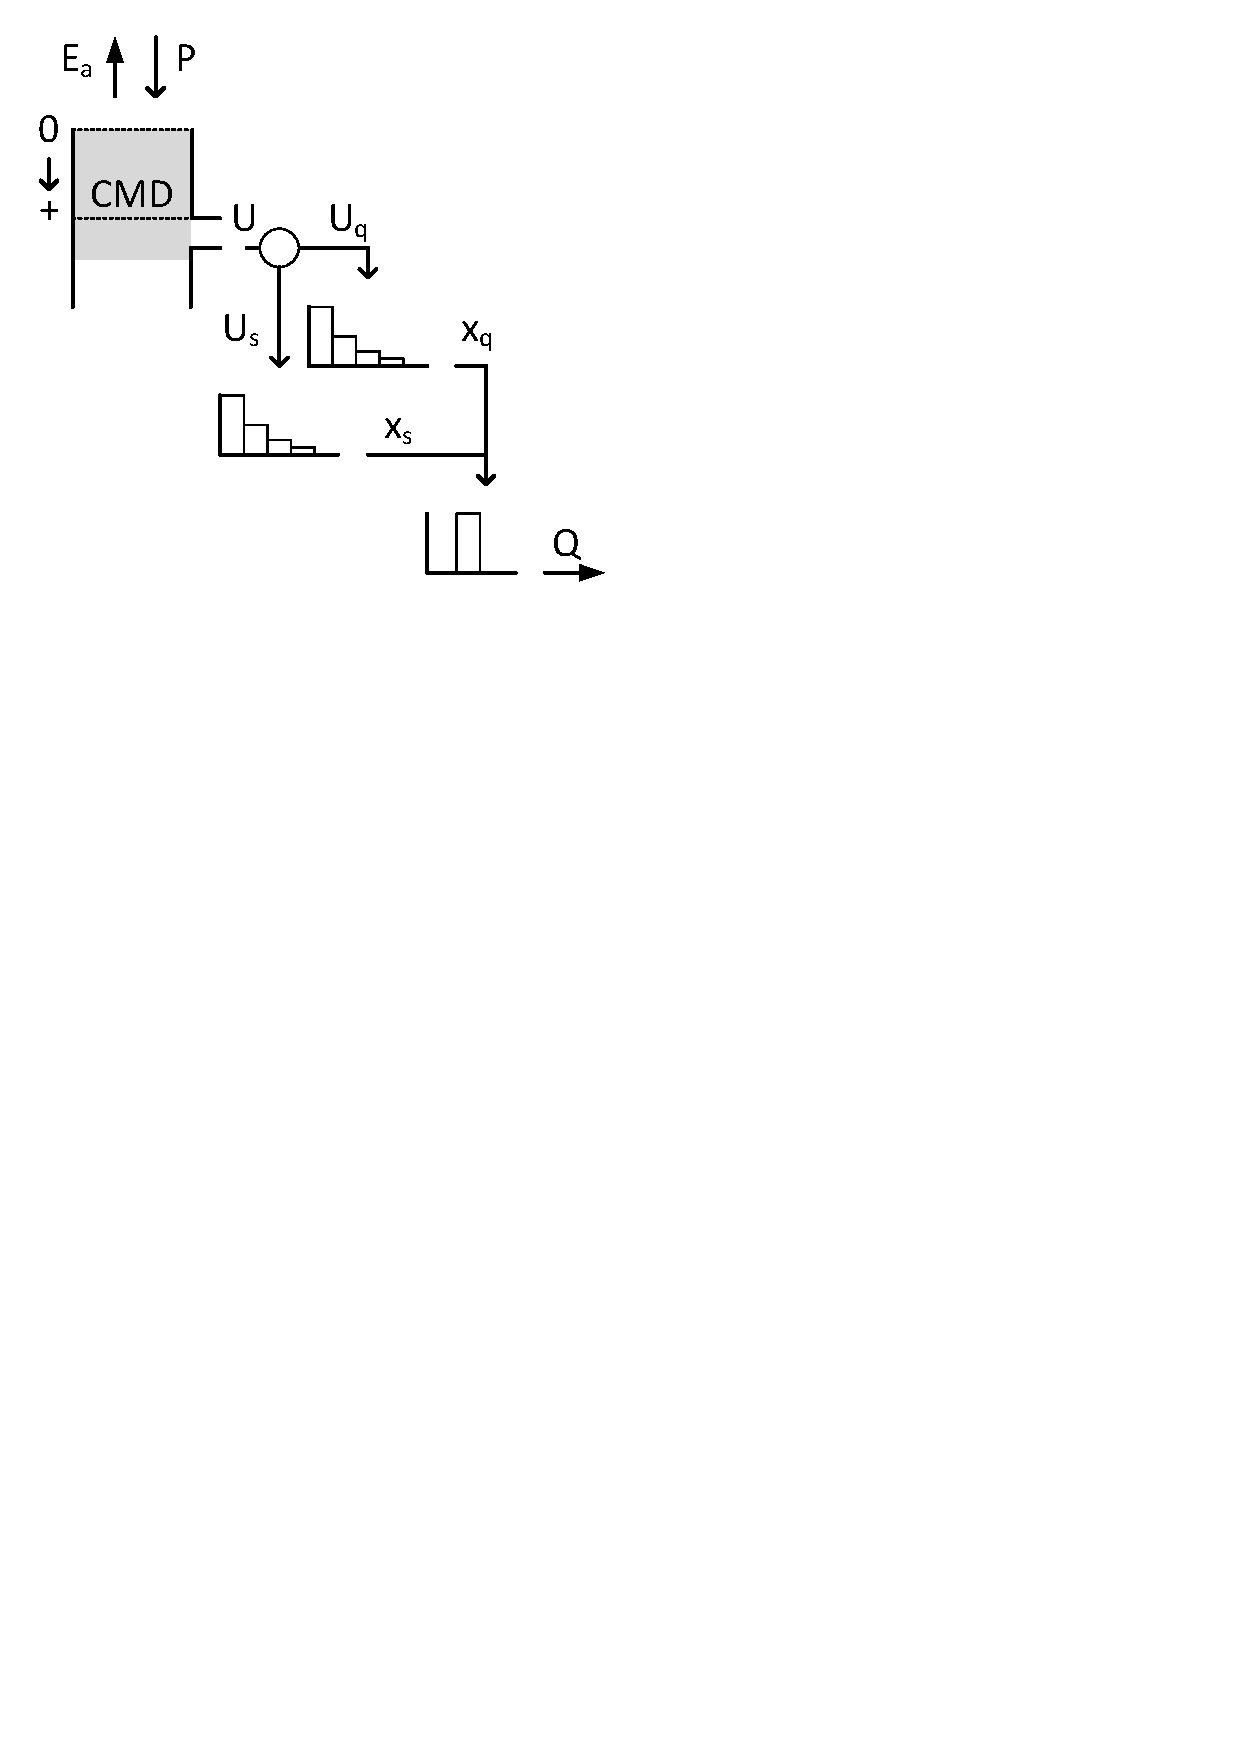
\includegraphics[trim=1cm 20cm 7cm 1cm,width=7cm,keepaspectratio]{./files/05_schematic.pdf}
\caption{Structure of the IHACRES model} \label{fig:05_schematic}
\end{wrapfigure}

\begin{align}
	\frac{dCMD}{dt} &= -P+E_a+U \\
	E_a &= E_p *min\left(1,e^{2\left(1-\frac{CMD}{lp}\right)}\right) \\
	U &= P\left(1-min\left(1,\left(\frac{CMD}{d}\right)^p\right)\right) \\
	U_q &= \alpha *U\\
	U_s &= (1-\alpha)*U
\end{align}

Where $CMD$ is the current moisture deficit [mm], $P$ $[mm/d]$ the incoming precipitation that \emph{reduces} the deficit, $E_a$ $[mm/d]$ evaporation that \emph{increases} the deficit, and $U$ $[mm/d]$ the effective precipitation that occurs when the deficit is below a threshold $d$ [mm], partly controlled by non-linearity parameter $p$ [-].

}

Evaporation occurs at the potential rate $E_p$ until the moisture deficit reaches wilting point $lp$ [mm], after which evaporation decreases exponentially with increasing deficit. Effective precipitation $U$ equals incoming precipitation $P$ when the deficit is zero, and decreases as a linear fraction of P until moisture deficit is larger than a threshold $d$ [mm], after which precipitation does not contribute to streamflow any longer. $U$ is divided between fast and slow routing components based on fraction $\alpha$ [-]. Both routing schemes are exponentially decreasing over time with lags $\tau_q$ [d] and $\tau_s$ [d] respectively. The total flow is given by:

\begin{align}
	Q &= x_q+x_s
\end{align}

which is optionally delayed with a pure time delay $\tau_d$ [d]. Note that this pure delay is not quite the same as the earlier Unit Hydrographs (specified by time base $\tau_q$ and $\tau_s$). The Unit Hydrographs \emph{transform} flow over a given number of time steps, whereas the delay $\tau_d$ \emph{delays} flow by a given number of time steps.

\subsubsection{Parameter overview}
% Table generated by Excel2LaTeX from sheet 'Sheet1'
\begin{table}[htbp]
  \centering
    \begin{tabular}{lll}
    \toprule
    Parameter & Unit  & Description \\
    \midrule
    $lp$  & $mm$  & Wilting point \\
    $d$   & $mm$  & Deficit threshold for flow from rain \\
    $p$   & $-$   & Deficit non-linearity \\
    $\alpha$ & $-$   & Fraction flow to quick routing \\
    $\tau_q$ & $d$   & Unit Hydrograph time base \\
    $\tau_s$ & $d$   & Unit Hydrograph time base \\
    $\tau_d$ & $d$   & Unit Hydrograph delay \\
    \bottomrule
    \end{tabular}%
  \label{tab:addlabel}%
\end{table}%


